\chapter{Modelado de los datos: ordenación de los usuarios}
\label{chap:ordenacion_de_usuarios}

\section{Principales hip\'otesis}
Una vez que ya tenemos una lista de usuarios cuyas publicaciones en Twitter
indican que podrían ser candidatos para las ofertas de trabajo, el siguiente
paso es ordenarlos por orden de relevancia. A continuación describimos brevemente
los dos criterios que usaremos para ordenarlos (el detalle de los algoritmos y 
procedimientos llevados a cabo en cada caso se hará en la secciones siguientes):
\begin{itemize}
\item Ordenación de tipo índice $h$. El índice h es un sistema propuesto por Jorge Hirsch, de la Universidad de California, para la medición de la calidad profesional de los científicos, en función de la cantidad de citas que han recibido sus artículos científicos\footnote{\url{https://en.wikipedia.org/wiki/H-index }}. Un científico tiene índice $h$ si ha publicado $h$ trabajos con al menos $h$ citas cada uno. El índice se diseñó para medir eficazmente la calidad del investigador, a diferencia de sistemas de medición más sencillos que cuentan citas o publicaciones, donde se hace una distinción entre aquellos investigadores que tienen una gran influencia en el mundo científico de aquellos que simplemente publican muchos trabajos. En nuestro campo, lo que queremos es medir 
la relevancia de los candidatos, así que una métrica de este tipo aplicada a los tuits publicados
de la temática de interés (Big Data y ciencia de datos en nuestro caso), nos ayudará a determinarla.
Los detalles, en la sección \ref{subsect:indice_h}.

\item Ordenación en función del papel de cada usuario dentro de la red de usuarios
seleccionados (sección \ref{subsect:grafo}). Para ello, construiremos el grafo 
de los candidatos y sus relaciones, siendo estas relaciones dirigidas (A está relacionado
con B si A sigue a B).
\end{itemize}

Con estos dos métodos pensamos que quedará bastante bien representado el panorama
de candidatos a partir de la información extraída de Twitter. 
Todos los cálculos descritos en esta parte del proyecto están en el archivo
{\bf ordenacion\_usuarios.py} del repositorio de GitHub.

\section{Algoritmos}
En esta sección detallamos los algoritmos que hemos usado para cada sistema de
clasificación, aportando la justificación de las diversas elecciones que 
hemos llevado a cabo.
\subsection{Índice h}
\label{subsect:indice_h}
La particularización del índice $h$ a nuestro contexto podría ser 
del siguiente modo: un usuario de Twitter tendrá índice $h$ si $h$ de sus $N$ tuits
sobre un determinado tema, han sido retuiteados al menos $h$ veces.

Calcular el índice $h$ implica por tanto los siguientes pasos:
\begin{enumerate}
\item Explorar el timeline\footnote{\lq\lq Timeline\rq\rq es la palabra
que usan en Twitter para referirse a un flujo de publicaciones a lo largo del tiempo.
El timeline de un usuario es el flujo de las publicaciones de ese usuario.} 
de cada usuario. Para ello usaremos la función
{\tt user\_timeline} que ofrece el paquete de Python {\tt Tweepy}. 
\item Determinar, dentro de ese timeline, qué tuits son del tema que nos interesa
(Big Data o ciencia de datos) y descartar el resto.
\item De cada tuit publicado sobre el tema de interés, anotar su número de 
retuits y calcular el índice $h$. 
\end{enumerate}

La descarga del timeline de usuarios tienen varias limitaciones en el acceso a través 
del API de Twitter\footnote{\url{https://developer.twitter.com/en/docs/tweets/timelines/api-reference/get-statuses-user_timeline }}:
\begin{itemize} 
\item límite de $1500$ llamadas por cada ventana de $15$ minutos,
\item solo se permite acceder a los $3200$ más recientes tuits de cada usuario,
\item el número de tuits descargados en cada llamada al API solo puede ascender a $200$.
\end{itemize}
Para que el proceso de obtención de datos no se pare cuando alcanzamos el límite
de llamadas (da un error), la función de {\tt Tweepy} permite incluir el parámetro 
{\tt wait\_on\_rate\_limit = True} para gestionar ese error y esperar a reanudar
el proceso cuando sea posible.

La función del API de Twitter para obtener el timeline de los usuarios no tiene 
la opción de buscar tuits de forma temporal (por ejemplo, los de los tres
últimos meses). Hemos optado por evaluar el timeline respecto a los últimos
$200$ tuits publicados por parecernos un número lo suficientemente amplio para 
el objetivo de clasificar los usuarios, si bien se podría incluir en el código la
gestión de un número mayor de tuits en el timeline (aumentando el número de
llamadas al API).

Un aspecto importante a la hora de evaluar el impacto del usuario es distinguir 
entre sus publicaciones originales y los retuits. De los tuits que componen el 
timeline, vamos a extraer la siguiente información:
\begin{itemize}
\item el número de tuits descargados(que 
en principio serán $200$, pero podrían ser menos),
\item el número de tuits sobre el tema de interés, y por tanto el
porcentaje de tuits de interés sobre el total de tuits evaluados,
\item sobre los tuits de interés, el porcentaje de aquellos que son retuits,
\item el índice $h$ de los tuits originales. Para calcular el índice $h$ 
contaremos tanto las veces que se ha retuiteado el tuit como las que ha sido
citado.
\end{itemize}

Al intentar bajar el timeline de algunos usuarios se pueden
obtener diversos mensajes de error (por ejemplo, porque el usuario tenga
protegido tu timeline, porque el usuario haya dejado de existir, etc.)
de forma que el proceso puede fallar. El código debe contemplar ese
caso y permitir que la ejecución continue con el resto de usuarios:

\myfigure{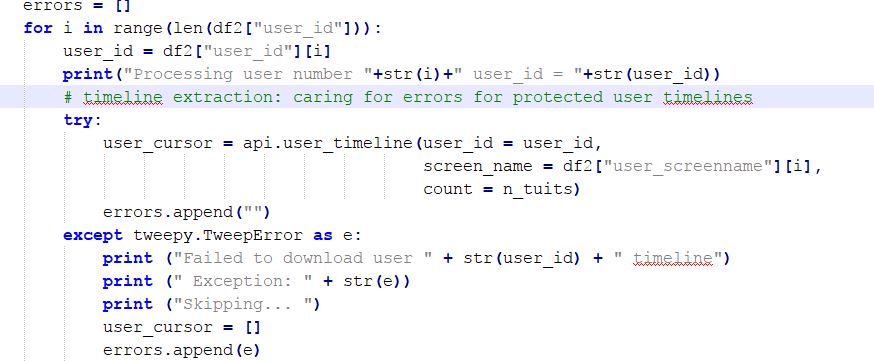
\includegraphics[width=0.6\textwidth]{error_not_authorized}%
\figcaption{Control de errores en la descarga de timelines.}
\label{fig:error_not_authorized} }


\subsection{Grafo relacional}
\label{subsect:grafo}
Nuestro objetivo en esta parte es explorar las relaciones entre los usuarios que 
hemos identificado como relevantes. De forma natural, como en cualquier red social,
se pueden definir multitud de estructuras de tipo grafo para describirlas. Nosotros
vamos a usar un grafo cuyos vértices serán los usuarios, y cuyas aristas o arcos serán
las relaciones entre ellos, de tipo dirigido: el usuario A está relacionado con el
usuario B si A sigue a B (y puede muy bien ocurrir que B no esté relacionado con A,
según esta definición). 

Para esta parte necesitaremos entonces descargar de Twitter la información
necesaria para construir el grafo de relaciones: los seguidores 
(\lq\lq followers\rq\rq\footnote{A aquellos usuarios que siguen a un determinado usuario, 
en Twitter se les denomina \lq\lq followers\rq\rq. Y se llaman \lq\lq friends\rq\rq aquellos
a los que dicho usuario determinado sigue.})
de cada uno de los usuarios identificados como potenciales candidatos. 
En principio, podríamos usar tanto los followers como los friends de cada uno 
de los usuarios de nuestra lista. Pero en realidad no hace falta, ya que si el usuario
A es un friend del usuario B, B es un follower del usario A, y lo consideraremos al
estudiar los followers de A. 

Para explorar los followers de cada usuario seleccionado usaremos la función 
{\tt followers\_ids} del paquete {\tt Tweepy}. Esta función es una interfaz
para la función del API de Twitter que permiten acceder a la lista de 
followers. Esta función del API de Twitter
tiene una limitación de $15$ llamadas al API por cada ventana de $15$ 
minutos\footnote{\url{https://developer.twitter.com/en/docs/accounts-and-users/follow-search-get-users/api-reference/get-followers-ids }},
con lo que la gestión de los límites es especialmente importante en este caso.
El parámetro {\tt wait\_on\_rate\_limit = True} al crear el acceso al API a 
través de {\tt Tweepy} también nos va a ser de utilidad.

Por otro lado, la información que puede descargarse con esa función también
está limitada en cantidad: el número de followers que puede obtenerse en cada llamada 
al API es a lo sumo $5000$. Igual que antes,
usando un código con varias llamadas al API, podríamos obtener un número más elevado de 
seguidores.

Nuestro grafo será por tanto un par ordenado 
$G=(N,g)$, donde $N$ es un conjunto de vértices o nodos, que serán los usuarios
identificados como potenciales candidatos para la oferta de trabajo, y $g$
 es un conjunto de aristas o arcos, descritos como pares de nodos ordenados:
$$g=\{(a,b): a,b\in N, a \mbox{ sigue a }b\}.$$
En las representaciones de un grafo dirigido, una relación $(a,b)$ se 
suele describir con una flecha que sale de $a$ y apunta a $b$.
Al extraer la información sobre los usuarios hemos de quedarnos con los followers
de cada uno que están en el conjunto de usuarios, es decir, solo nos quedamos con
las relaciones entre candidatos:

\myfigure{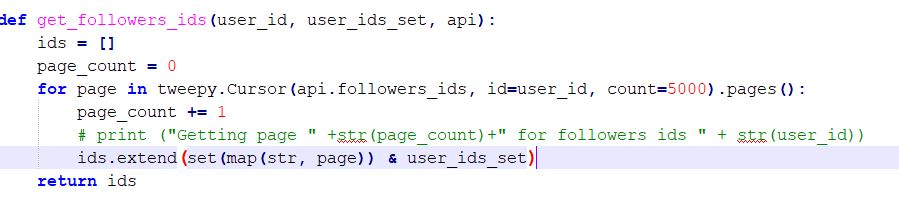
\includegraphics[width=0.8\textwidth]{followers_code}%
\figcaption{Followers y relación entre usuarios.}
\label{fig:followers_code} }

Una vez obtenidas estas relaciones, vamos a necesitar una librería 
para procesar el grafo y sacar las pertinentes 
conclusiones. A este respecto, tenemos varias opciones que 
considerar. Entre otras:
\begin{itemize}
\item {\tt Graph-tool}: los algoritmos están implementadas en una librería C++, 
lo que aporta mucha rapidez en la ejecución. Es 
buena procesando grafos grandes. La instalación en entornos Windows no
está soportada\footnote{\url{https://git.skewed.de/count0/graph-tool/wikis/installation-instructions 
}}.
\item {\tt NetworkX} es fácil de usar, para conjuntos de datos pequeños. Está bien
documentado. Es compatible con Python 2.7, 3.4, 3.5 y 3.6.
\item {\tt SNAP} (Stanford Network Analysis Platform): es un sistema para el análisis
y la manipulación de grandes redes. Está implementada en C++, con una interfaz en Python. 
Disponible para Python 2.7\footnote{\url{https://snap.stanford.edu/snappy/index.html }}.
\item {\tt igraph}: es una colección de herramientas para análisis de grafos,
con interfaces en R, Python y C/C++. Compatible con Python 2.6, 2.7 y 3.2.
\item {\tt APGL} (Another Python Graph Library): es una librería sencilla
para procesar grafos, disponible en principio para Python 2.7\footnote{\url{https://pythonhosted.org/apgl/ }}.
\end{itemize}

Vistas las opciones, nos hemos decidido por usar {\tt NetworkX}.
Esta herramienta nos va a permitir calcular varias medidas
de interés para estudiar la red de usuarios (\cite{notas_fernando}):
\begin{itemize}
\item Para entender la proximidad de unos nodos con otros:
\begin{itemize}
\item Diámetro: la mayor distancia geodésica dentro del grafo (o componente si no es conexo)
\item Camino mínimo: camino más corto entre 2 nodos
\item Longitud del camino medio: media de todos los caminos mínimos entre los 
nodos del grafo (menos sensible a valores extremos).
\end{itemize}
\end{itemize}
Y también usaremos el grafo para estudiar el papel de cada usuario dentro de la red
y medir su relevancia, calculando las siguientes métricas:
\begin{itemize}
\item Centralidad por grado: el grado (degree) de un nodo $n$ es el número de aristas 
incidentes en $n$. En los grafos dirigidos podemos distinguir entre in-degree (número
de aristas que apuntan a $n$, en nuestro caso el número de followers) y
out-degree (número de aristas que parten de $n$, en nuestro caso, el número de
usuarios a los que sigue $n$). El in-degree representaría la capacidad de 
\lq\lq liderazgo\rq\rq
del usuario (a más followers, en principio más liderazgo), y el out-degree 
representaría el interés del usuario en seguir a otros usuarios, que podríamos
interpretar como su interés por el clima general del sector.
\item Centralidad por autovector (eigenvector centrality): es una extensión del 
concepto de cen\-tra\-li\-dad por grado que captura la intuición de que la importancia 
de un nodo en la red incrementa por el hecho de estar conectado a otros nodos 
a su vez relevantes. En un grafo dirigido como el nuestro, parece natural pensar que
lo que debemos medir es la importancia de los usuarios que siguen a uno dado,
y que por tanto deberíamos usar los enlaces que apuntan al usuario en cuestion (las 
aristas que cuentan para el in-degree).  Sea $c$ el vector columna
de las centralidades por autovector de los $n$ nodos del grafo y sea $A$ la matriz
de adyacencia del grafo, en la que $a_{ij}$ representa la contribución
del nodo $n_i$ al \lq\lq prestigio\rq\rq del nodo $n_j$ (en nuestro caso, $a_{ij} = 1$ si
$n_i$ sigue a $n_j$ y cero en caso contrario). La idea detrás de esta centralidad
(\cite{bonacich2}) es que la centralidad de un nodo será la suma de las centralidades
de los nodos que le apuntan, ponderadas por el peso de la unión, esto es:
$$c_i = \sum_j a_{ji} c_j$$
que en notación matricial es 
$$c = A^Tc.$$
Para que esta ecuación tenga solución debemos considerar una formulación más general,
en la que la centralidad no es exactamente la suma de las centralidades de los nodos que 
contribuyen, sino solo un múltiplo de dicha suma:
$$\lambda c = A^Tc,$$
de tal forma que $c$, el vector de las centralidades del grafo es un 
autovector de la matriz $A^T$. Si $A$ es una matriz $n\times n$ hay en general $n$ soluciones
a dicha ecuación, correspondientes a los $n$ autovalores de $A^T$. Suele considerarse
como solución favorita el autovector correspondiente al máximo autovalor.
 
\item Centralidad de Bonacich: la centralidad por autovector tiene un problema cuando
alguno de los nodos no tiene enlaces que lo apunten (es decir, si alguno de los usuarios
no tuviera ningún seguidor entre los demás usuarios, aunque él sí que siguiera a otros),
ya que en ese caso ese nodo siempre contribuirá cero, y por tanto, en algunos casos
la centralidad por autovector de todos los nodos sería cero (ejemplos I y II de la página
192 de \cite{bonacich}). Para
paliar este problema podemos usar la centralidad de Bonacich, que  parte de la siguiente
idea: todos los nodos tienen centralidad mínima. Con la misma notación que en el apartado
anterior, la centralidad de Bonacich puede definirse 
(ecuación $(5)$ en \cite{bonacich}) como:
$$c_i = e_i + \alpha\sum_j a_{ji} c_j, \mbox{ o, en notación matricial, } c = e + \alpha A^Tc$$
donde $\alpha\in[0,1]$ y $e$ es un vector constante. Esto es, la centralidad de cada nodo es la suma
de una centralidad mínima (o exógena, como la denominan en \cite{bonacich}) 
y de las contribuciones a la centralidad de las centralidades de los nodos que apuntan 
a dicho nodo. Esa contribución se amortigua a través del parámetro $\alpha$, 
ya que para nodos a distancia $k$ de un nodo dado, su contribución es múltiplo de
$\alpha^k$. Si $\alpha=0$, no hay transmisión de centralidad.
\item PageRank: las centralidades basadas en autovectores distribuyen de forma indiscriminada 
su centralidad a todos sus vecinos,  por lo que un nodo importante que apunta a 
muchos vecinos hace importantes a todos ellos. La idea de PageRank consiste en 
repartir la centralidad aportada por un nodo entre todos sus vecinos. De esta forma, si un nodo muy importante apunta a muchos 
nodos, finalmente la centralidad que recibe cada uno de ellos quede diluida.
La centralidad que un nodo recibe de cada vecino de su red, es 
centralidad vecino / outdegree
PageRank es un proceso iterativo, hasta que se completa un ciclo y los valores no 
cambian, la solución converge. (o hasta que se completa un máximo de ciclos)
\end{itemize}


\section{Almacenamiento}